
%Wzbudzalnosc w sekcji dyspersja

\subsection{Wyznaczanie krzywych wzbudzalności}

Krzywe wzbudzalności określają zależność amplitudy od częstotliwości fali dla poszczególnych jej modów i dla danego wymuszenia. Dla pewnych przypadków można wyznaczyć taką zależność analitycznie, jednak podobnie jak w przypadku krzywych dyspersji, nie jest to metoda uniwersalna. Poniżej znajdują się wyłącznie przykładu numerycznych sposobów wyznaczania tego typu krzywych, ponieważ mają one szersze zastosowanie.

Pierwszy sposób wykorzystuję standardowy model MES ze wzoru \ref{eq:MES1}. Wyznaczamy przemieszczenia węzłów w pewnych chwilach czasowych , a następnie obliczamy wielowymiarowe przekształcenie Fouriera na zgromadzonych danych \ref{eq:fourier_2d}. Wynikiem transformacji jest zależność częstości i liczby falowej, co pozwala wykreślać krzywe dyspersji, a dodatkowo trzecia oś, prostopadła do pozostałych, zawiera informacje o amplitudzie. Przedstawiając na płaszczyźnie zależność amplitudy od liczby falowej, otrzymamy krzywe wzbudzalności.

\vspace{3mm}

Innym sposobem omawianym w literaturze jest zastosowanie metody SAFE (Semi-Analytical Finite Element). Jest ona modyfikacją metody elementów skończonych, polegającą na ustaleniu analitycznego rozwiązania problemu, dla jednego kierunku propagacji. W przypadku problemu trójwymiarowego pozwala to na tworzenie elementów dwuwymiarowych, w kierunkach propagacji, dla których nie znamy rozwiązania. Dzięki temu cały model jest prostszy i szybszy w rozwiązaniu. Sformułowanie takie jest jednak złożone i nie będzie tutaj przytaczane w całości. Jest ono opisane dokładniej w \cite{bartek_fabien}.

Wynikiem wykorzystania metody SAFE jest związek siły wymuszającej i przemieszczenia węzłów modelu. Związek ten przedstawia wzór \ref{eq:wzbudzanie1}. Wzbudzalność określić można na podstawie macierzy E. Określa ona dla modu m, związek pomiędzy siłą przyłożoną w i-tym węźle i przemieszczeniu j-tego węzła \( (\textbf{E}_m)_{ij} \). Rysunek \ref{fig:wzbudzalnosc1} przedstawia wzbudzalność obliczoną dla pierwszych dwóch modów w dwuwarstwowej płycie, bez tłumienia.

\begin{equation} \label{eq:wzbudzanie1}
\textbf{U} = \sum_{m=1}^M \textbf{E}_m \textbf{F}(k_m) e^{ik_m z}
\end{equation}

gdzie
\begin{eqwhere}[2cm]
	\item[$U$] wektor przemieszczenia węzłów
	\item[$E$] macierz wzbudzalności
	\item[$U$] siła wymuszająca w dziedzinie liczby falowej
	\item[$z$] kierunek propagacji, dla którego założono rozwiązanie analityczne
	\item[$m$] numer modu
	\item[$M$] liczba propagujących modów
	\item[$k$] liczba falowa dla m-tego modu.	
\end{eqwhere}

\begin{figure}[h]
\centering
\includegraphics[width=10cm]{Zdjecia/2/wzbudzalnosc1}
\caption{Krzywe wzbudzalności dla dwuwarstwowej cienkiej płyty \cite{bartek_fabien}}
\label{fig:wzbudzalnosc1}
\end{figure}

Kolejna metoda polega na porównaniu prac modów dla fal Lamba z tzw. modem wirtualnym . Prowadzi ona do zależności na wzbudzalność dla cienkich płyt:

\begin{equation} \label{eq:wzbudzanie2}
a_m =  \textbf{X}_m^{(b), H} \frac{\textbf{F}(z)}{i\textbf{P}_{(a:m),(b)}}.
\end{equation}

gdzie

%\begin{equation} \label{eq:wzbudzanie2}
%P_{(a:m),(b)} = \textbf{X}_m^{(b), H} (\textbf{K}_{+1}^{(b),H} e^{-k^{(b)}\Delta x} - \textbf{K}_{-1}^{(b),H} e^{+ik^{(b)}\Delta x} - \textbf{K}_{+1}^{(a)} e^{+ik_m^{(a)}\Delta x} + \textbf{K}_{-1}^{(a)} e^{-ik_m^{(a)}\Delta x})\textbf{X}_{0,m}^{(a)} = 0
%\end{equation}

\begin{equation} \label{eq:wzbudzanie3}
\textbf{P}_{(a:m),(b)} = \textbf{X}_m^{H} (\textbf{K}_{+1}^{H} e^{-ik\Delta x} - \textbf{K}_{-1}^{H} e^{+ik\Delta x} - \textbf{K}_{+1} e^{+ik\Delta x} + \textbf{K}_{-1} e^{-ik\Delta x})\textbf{X}_{0}
\end{equation}

\begin{eqwhere}[2cm]
	\item[$a_m$] amplituda m-tego modu w odpowiedzi na wymuszenie
	\item[$\textbf{F}(z)$] siła wymuszająca działająca wzdłuż grubości płyty
	\item[$\textbf{X}$] wektory własne 
	\item[$\textbf{K}_{\pm 1}$] macierz sztywności dla kolejnej/poprzedniej płaszczyzny propagacji
	\item[$k$] liczba falowa
	\item[$x$] kierunek propagacji
	\item[$m$] numer modu	
	\item[$a_m$] mod numer m, dla pola falowego a
	\item[$b$] mod wirtualny b	
	\item[$H$] sprzężenie hermitowskie.
\end{eqwhere}

Należy zaznaczyć, że do obliczenia amplitud poszczególnych modów, konieczna jest znajomość krzywych dyspersji (zależności \( k(\omega) \) ), oraz wektorów własnych odpowiadających częstościom własnym, dla których wyznaczamy amplitudy.

\subsection{System sing\_around (lub Self-Excited Acoustical System)}

Systemy sing-around to samowzbudne systemy, do pomiaru parametrów rezonansowych fal. Idea systemu polega na dodatnim sprzężeniu zwrotnym pomiędzy przetwornikiem pomiarowym oraz wzbudnikiem. Badanie konstrukcji rozpoczyna arbitralny sygnał wzbudzający. Przetwornik pomiarowy odbiera sygnał i przetwarza go na sygnał elektryczny, który jest odpowiednio filtrowany i wzmacniany, a następnie podawany do wzbudnika. Dane pomiarowe są przesyłane do systemu akwizycji i obróbki, w celu wydobycia informacji o stanie konstrukcji. Schemat przykładowego stanowiska badawczego znajduje się na rysunku \ref{fig:sing_around}.

\begin{figure}[h]
\centering
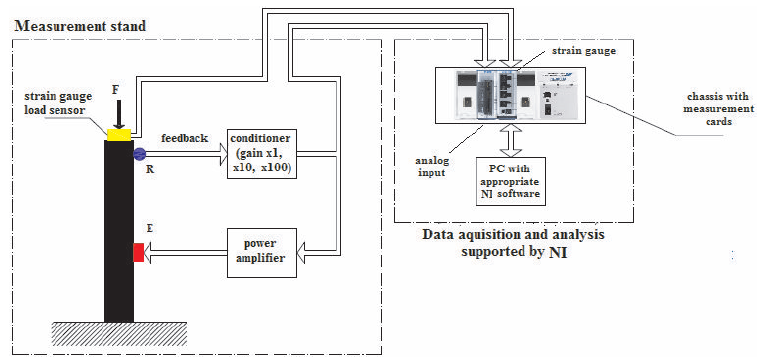
\includegraphics[width=10cm]{Zdjecia/2/sing_around}
\caption{Stanowisko badawcze z systemem sing around \cite{bartek_kwach}}
\label{fig:sing_around}
\end{figure}

Popularnym zastosowaniem tego typu systemów jest pośredni pomiar naprężeń, które mają związek z częstotliwością rezonansową układu bądź prędkością fali, które zmieniają się wraz z odkształcaniem się materiału. Praktycznym przykładem jest pomiar częstotliwości rezonansowej słupa podporowego silosa cementu. Na rysunkach \ref{fig:sing_around_silos} i \ref{fig:sing_around_wyniki} znajduje się widok stanowiska pomiarowego oraz wyniki pomiarów, dla zwiększania i zmniejszania się masy cementu w silosie. W ciągu minuty do silosa dostarczane jest 500kg cementu (125 kg na podporę), a jedno rozładowanie to ok. 2500kg (625 kg na podporę). Przedstawione wyniki dotyczą konfiguracji E1, R1, gdzie E1 to wzbudnik, a R1 to przetwornik pomiarowy.

\begin{figure}[h]
\centering
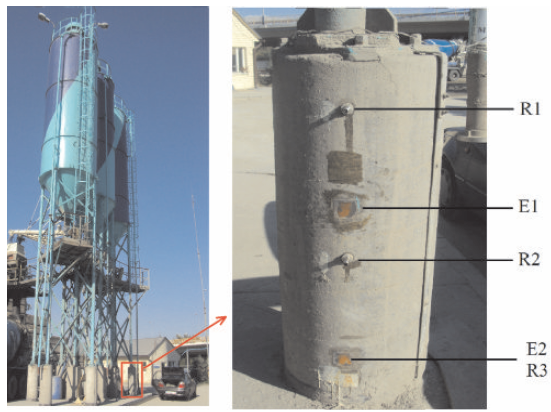
\includegraphics[width=10cm]{Zdjecia/2/sing_around_silos}
\caption{Widok podpory silosa z zamontowanymi przyżadami \cite{bartek_kwach}}
\label{fig:sing_around_silos}
\end{figure}

\begin{figure}[h]
\centering
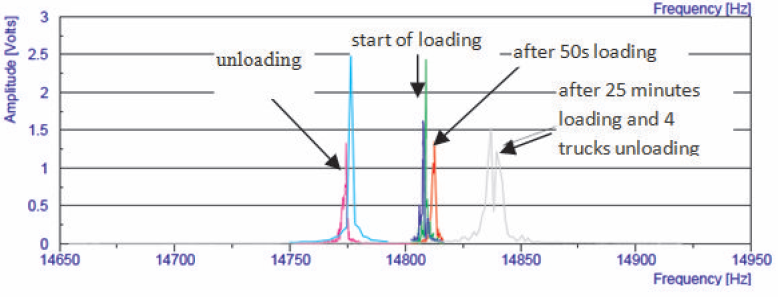
\includegraphics[width=14cm]{Zdjecia/2/sing_around_wyniki}
\caption{Wyniki pomiaru dla ciągłego dostarczania cementu do silosa \cite{bartek_kwach}}
\label{fig:sing_around_wyniki}
\end{figure}

Jak widać częstotliwość rezonansowa zwiększa się wraz ze wzrostem naprężeń ściskających w badanej podporze. Tego typu systemy mają ogromne możliwości zastosowań w różnego typu konstrukcjach, gdzie istotne jest monitorowanie naprężeń.

Znajomość krzywych dyspersji oraz krzywych wzbudzalności dla określonego wymuszenia pozwala zasymulować działanie układu sing-around. Sygnał wyjściowy dla symulacji przebiegu fali, należy podać jako wejście do kolejnej symulacji. Uwzględnienie krzywych dyspersji pozwala określić sposób pomiaru, dla sygnału, który rozbiega się w czasie. Krzywe wzbudzalności pozwalają wyznaczyć piki rezonansowe w widmie badanego sygnału.

